% !TEX program = xelatex

\documentclass[10pt, aspectratio=169]{beamer}

\usetheme[progressbar=none, numbering=none]{metropolis}
\usepackage{xcolor}
\usepackage{tikz}
\usetikzlibrary{calc,positioning}

% Paleta visual: industrial, escura, com acentos de sinal.
\definecolor{BaseBg}{HTML}{0B1020}
\definecolor{TopBar}{HTML}{111827}
\definecolor{PanelBg}{HTML}{172033}
\definecolor{PanelEdge}{HTML}{233047}
\definecolor{GridLine}{HTML}{26344F}
\definecolor{TextPrimary}{HTML}{F8FAFC}
\definecolor{TextMuted}{HTML}{AAB6C8}
\definecolor{AccentCyan}{HTML}{16D5D2}
\definecolor{SignalGreen}{HTML}{7DDC8A}
\definecolor{SignalAmber}{HTML}{F7B955}

\setbeamercolor{background canvas}{bg=BaseBg}
\setbeamercolor{normal text}{fg=TextPrimary,bg=BaseBg}
\setbeamercolor{frametitle}{fg=TextPrimary,bg=TopBar}
\setbeamercolor{title}{fg=TextPrimary}
\setbeamercolor{subtitle}{fg=TextMuted}
\setbeamercolor{author}{fg=TextMuted}
\setbeamercolor{institute}{fg=TextMuted}
\setbeamercolor{date}{fg=SignalAmber}
\setbeamercolor{alerted text}{fg=AccentCyan}
\setbeamercolor{block title}{fg=TextPrimary,bg=PanelEdge}
\setbeamercolor{block body}{fg=TextPrimary,bg=PanelBg}
\setbeamercolor{footline}{fg=TextMuted,bg=BaseBg}

\setbeamerfont{title}{size=\LARGE,series=\bfseries}
\setbeamerfont{subtitle}{size=\large}
\setbeamerfont{frametitle}{size=\large,series=\bfseries}
\setbeamerfont{block title}{series=\bfseries}
\setbeamerfont{footline}{size=\scriptsize}

\setbeamertemplate{navigation symbols}{}
\setbeamertemplate{blocks}[rounded][shadow=false]
\setbeamertemplate{itemize item}{\tikz\fill[AccentCyan] (0,0) circle (1.9pt);}
\setbeamertemplate{itemize subitem}{\tikz\fill[SignalGreen] (0,0) rectangle (3pt,3pt);}

% Fundo tecnico discreto: grade fina e planos de profundidade.
\setbeamertemplate{background}{
    
\begin{tikzpicture}
        \useasboundingbox (0,0) rectangle (\paperwidth,\paperheight);
        \fill[BaseBg] (0,0) rectangle (\paperwidth,\paperheight);

        \foreach \x in {0,0.55,...,16.6} {
            \draw[GridLine, opacity=0.18, line width=0.2pt] (\x,0) -- (\x,\paperheight);
        }
        \foreach \y in {0,0.55,...,9.4} {
            \draw[GridLine, opacity=0.18, line width=0.2pt] (0,\y) -- (\paperwidth,\y);
        }

        \fill[PanelBg, opacity=0.34] (12.45,0) -- (\paperwidth,0) -- (\paperwidth,\paperheight) -- (14.35,\paperheight) -- cycle;
        \draw[AccentCyan, opacity=0.18, line width=0.8pt] (12.55,0) -- (14.45,\paperheight);
        \draw[SignalGreen, opacity=0.16, line width=0.8pt] (13.25,0) -- (15.15,\paperheight);
        \fill[AccentCyan, opacity=0.22] (0,0) rectangle (\paperwidth,0.055);
    \end{tikzpicture}
}

\setbeamertemplate{frametitle}{
    \nointerlineskip
    \begin{beamercolorbox}[wd=\paperwidth,ht=0.95cm,dp=0.28cm,leftskip=0.82cm,rightskip=0.75cm]{frametitle}
        \usebeamerfont{frametitle}\insertframetitle
    \end{beamercolorbox}
    \begin{tikzpicture}[remember picture,overlay]
        \fill[AccentCyan] (current page.north west) rectangle ([xshift=0.16cm,yshift=-1.23cm]current page.north west);
        \fill[SignalGreen] ([xshift=0.16cm]current page.north west) rectangle ([xshift=0.23cm,yshift=-1.23cm]current page.north west);
        \draw[AccentCyan, opacity=0.5, line width=0.4pt] ([yshift=-1.23cm]current page.north west) -- ([yshift=-1.23cm]current page.north east);
    \end{tikzpicture}
}

\setbeamertemplate{footline}{
    \ifnum\value{framenumber}=1
    \else
        \begin{beamercolorbox}[wd=\paperwidth,ht=0.32cm,dp=0.16cm,leftskip=0.85cm,rightskip=0.85cm]{footline}
            \insertshorttitle\hfill\insertframenumber/\inserttotalframenumber
        \end{beamercolorbox}
    \fi
}

\setbeamertemplate{title page}{
    \begin{tikzpicture}[remember picture,overlay]
        \fill[AccentCyan] (current page.north west) rectangle ([xshift=0.18cm]current page.south west);
        \fill[SignalGreen] ([xshift=0.18cm]current page.north west) rectangle ([xshift=0.25cm]current page.south west);
        \fill[SignalAmber] ([xshift=0.25cm]current page.north west) rectangle ([xshift=0.30cm]current page.south west);

        \draw[AccentCyan, opacity=0.32, line width=1.1pt] ([xshift=0.85cm,yshift=-1.02cm]current page.north west) -- ([xshift=4.8cm,yshift=-1.02cm]current page.north west);
        \draw[SignalGreen, opacity=0.30, line width=1.1pt] ([xshift=0.85cm,yshift=-1.22cm]current page.north west) -- ([xshift=3.4cm,yshift=-1.22cm]current page.north west);
        \draw[SignalAmber, opacity=0.28, line width=1.1pt] ([xshift=0.85cm,yshift=-1.42cm]current page.north west) -- ([xshift=2.3cm,yshift=-1.42cm]current page.north west);

        \node[anchor=south east, text=PanelEdge, opacity=0.42, font=\fontsize{46}{46}\selectfont\bfseries]
            at ([xshift=-0.55cm,yshift=0.58cm]current page.south east) {PROFINET};
        \draw[PanelEdge, opacity=0.42, line width=0.5pt]
            ([xshift=-5.9cm,yshift=1.03cm]current page.south east) rectangle
            ([xshift=-0.65cm,yshift=2.08cm]current page.south east);
    \end{tikzpicture}

    \vspace*{1.35cm}
    \begin{minipage}{0.78\paperwidth}
        {\usebeamerfont{title}\usebeamercolor[fg]{title}\inserttitle\par}
        \vspace{0.28cm}
        {\usebeamerfont{subtitle}\usebeamercolor[fg]{subtitle}\insertsubtitle\par}
        \vspace{0.72cm}
        {\usebeamerfont{author}\usebeamercolor[fg]{author}\insertauthor\par}
        \vspace{0.10cm}
        {\usebeamerfont{institute}\usebeamercolor[fg]{institute}\insertinstitute\par}
        \vspace{0.35cm}
        {\usebeamerfont{date}\usebeamercolor[fg]{date}\insertdate\par}
    \end{minipage}
}

\newcommand{\slidechip}[2]{%
    \tikz[baseline=(chip.base)]\node[
        fill=#1,
        text=BaseBg,
        rounded corners=1.5pt,
        inner xsep=5pt,
        inner ysep=2pt,
        font=\scriptsize\bfseries
    ] (chip) {#2};%
}

\newcommand{\routebox}[3]{%
    \begin{tikzpicture}
        \node[
            fill=#1,
            text=TextPrimary,
            rounded corners=2pt,
            minimum width=2.65cm,
            minimum height=0.82cm,
            align=center,
            font=\footnotesize\bfseries
        ] {#2\\[-1pt]{\scriptsize #3}};
    \end{tikzpicture}%
}

% Informacoes da apresentacao
\title[PROFINET]{Pr\'atica: PROFINET e An\'alise de Tr\'afego}
\subtitle{Introdu\c{c}\~ao \`as Redes de Comunica\c{c}\~ao}
\author{Gabriel Silva}
\institute{Universidade Federal de Pernambuco (UFPE)}
\date{Semestre 2025.2}

\begin{document}

\begin{frame}
    \titlepage
\end{frame}

\begin{frame}{Objetivo da Pr\'atica}
    \begin{columns}[T,totalwidth=\textwidth]
        \begin{column}{0.46\textwidth}
            \begin{block}{Construir}
                Configurar dois CLPs S7-1500 em uma comunica\c{c}\~ao \alert{PROFINET RT}, com um controlador e um I-Device.
            \end{block}
        \end{column}
        \begin{column}{0.46\textwidth}
            \begin{block}{Comprovar}
                Capturar no Wireshark os pacotes de configura\c{c}\~ao \texttt{pn\_dcp} e os pacotes de tempo real \texttt{pn\_rt}.
            \end{block}
        \end{column}
    \end{columns}

    \vspace{0.45cm}
    \begin{block}{Ideia central da aula}
        O PROFINET usa o mesmo cabo para tr\'afego comum de rede e tr\'afego industrial determin\'istico. A diferen\c{c}a aparece claramente quando olhamos o frame Ethernet.
    \end{block}
\end{frame}

\begin{frame}{Mapa da Monitoria}
    \small
    \begin{columns}[T,totalwidth=\textwidth]
        \begin{column}{0.46\textwidth}
            \begin{block}{Pr\'atica no TIA Portal}
                \begin{itemize}
                    \item Criar projeto e adicionar os dois CLPs.
                    \item Configurar IPs e sub-rede \texttt{PN/IE\_1}.
                    \item Definir o segundo CLP como \textit{I-Device}.
                    \item Criar \textit{Transfer areas}.
                    \item Atribuir \textit{Device Name} via DCP.
                    \item Fazer download e validar em RUN.
                \end{itemize}
            \end{block}
        \end{column}
        \begin{column}{0.46\textwidth}
            \begin{block}{Teoria observada no Wireshark}
                \begin{itemize}
                    \item Modelo OSI na pr\'atica.
                    \item Canal ac\'iclico vs. canal c\'iclico.
                    \item DCP, MAC, multicast e limita\c{c}\~oes do DHCP.
                    \item PROFINET RT sem IPv4.
                    \item QoS com VLAN 802.1Q e prioridade 6.
                \end{itemize}
            \end{block}
        \end{column}
    \end{columns}
\end{frame}

\begin{frame}{Fase 1: Projeto e Topologia}
    \small
    \slidechip{AccentCyan}{TIA Portal}\hspace{0.25cm}
    \slidechip{SignalGreen}{Topologia}\hspace{0.25cm}
    \slidechip{SignalAmber}{Endere\c{c}amento}

    \vspace{0.35cm}
    \begin{columns}[T,totalwidth=\textwidth]
        \begin{column}{0.46\textwidth}
            \begin{block}{Conex\~ao f\'isica}
                \begin{itemize}
                    \item CLP 1, CLP 2 e computador no mesmo switch.
                    \item Cabo Ethernet comum, mesma rede local.
                    \item Abrir o TIA Portal e criar um novo projeto.
                \end{itemize}
            \end{block}
        \end{column}
        \begin{column}{0.46\textwidth}
            \begin{block}{Dispositivos no projeto}
                \begin{itemize}
                    \item Adicionar o modelo exato do primeiro S7-1500.
                    \item Renomear para \texttt{CLP\_Controlador}.
                    \item Adicionar o segundo S7-1500.
                    \item Renomear para \texttt{CLP\_IDevice}.
                \end{itemize}
            \end{block}
        \end{column}
    \end{columns}
\end{frame}

\begin{frame}{Endere\c{c}amento IP no TIA Portal}
    \small
    \begin{block}{\texttt{CLP\_Controlador}}
        \texttt{Device configuration} $\rightarrow$ porta PROFINET verde $\rightarrow$
        \texttt{Properties > Ethernet addresses} $\rightarrow$ IP \texttt{192.168.0.3}.
    \end{block}

    \begin{block}{Sub-rede industrial}
        Criar a sub-rede \texttt{PN/IE\_1} em \texttt{Add new subnet}.
    \end{block}

    \begin{block}{\texttt{CLP\_IDevice}}
        Repetir o caminho na porta PROFINET, definir IP \texttt{192.168.0.2} e conectar \`a mesma \texttt{PN/IE\_1}.
    \end{block}
\end{frame}

\begin{frame}{Teoria: Por Que Configurar IP?}
    \small
    \begin{block}{Pergunta para a turma}
        Se o PROFINET de tempo real n\~ao usa endere\c{c}o IP, por que o TIA Portal exige IPs na mesma sub-rede?
    \end{block}

    \vspace{0.25cm}
    \begin{columns}[T,totalwidth=\textwidth]
        \begin{column}{0.46\textwidth}
            \begin{block}{Canal ac\'iclico}
                \begin{itemize}
                    \item Usa IP e TCP/UDP.
                    \item Serve para download, diagn\'ostico e acesso web.
                    \item \'E tr\'afego de melhor esfor\c{c}o, sujeito a jitter.
                \end{itemize}
            \end{block}
        \end{column}
        \begin{column}{0.46\textwidth}
            \begin{block}{Canal c\'iclico}
                \begin{itemize}
                    \item Pula IP e TCP/UDP.
                    \item Vai de Ethernet diretamente para PROFINET RT.
                    \item Carrega dados cr\'iticos de controle.
                \end{itemize}
            \end{block}
        \end{column}
    \end{columns}
\end{frame}

\begin{frame}{OSI na Rede Industrial}
    \small
    \centering
    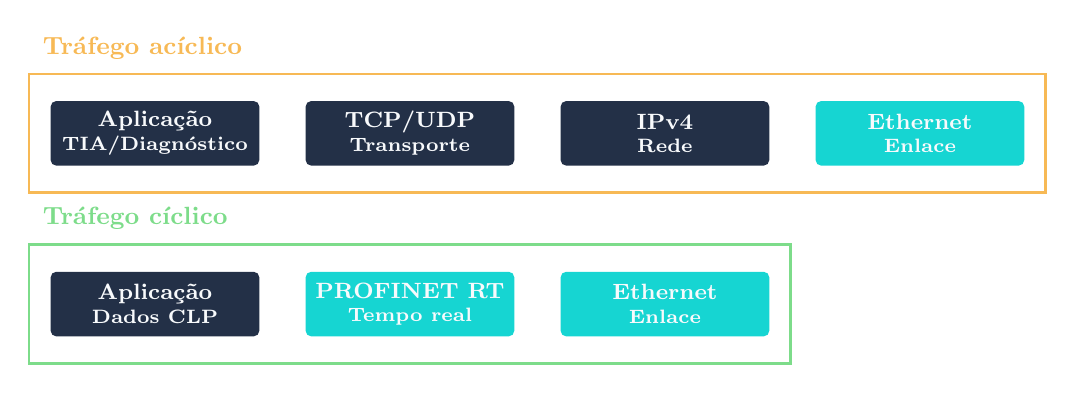
\begin{tikzpicture}[node distance=0.32cm]
        \node (a1) {\routebox{PanelEdge}{Aplica\c{c}\~ao}{TIA/Diagn\'ostico}};
        \node[right=0.34cm of a1] (a2) {\routebox{PanelEdge}{TCP/UDP}{Transporte}};
        \node[right=0.34cm of a2] (a3) {\routebox{PanelEdge}{IPv4}{Rede}};
        \node[right=0.34cm of a3] (a4) {\routebox{AccentCyan}{Ethernet}{Enlace}};

        \node[below=1.1cm of a1] (b1) {\routebox{PanelEdge}{Aplica\c{c}\~ao}{Dados CLP}};
        \node[right=0.34cm of b1] (b2) {\routebox{AccentCyan}{PROFINET RT}{Tempo real}};
        \node[right=0.34cm of b2] (b3) {\routebox{AccentCyan}{Ethernet}{Enlace}};

        \draw[SignalAmber, line width=1pt] ($(a1.north west)+(-0.15,0.22)$) rectangle ($(a4.south east)+(0.15,-0.22)$);
        \draw[SignalGreen, line width=1pt] ($(b1.north west)+(-0.15,0.22)$) rectangle ($(b3.south east)+(0.15,-0.22)$);
        \node[anchor=west, text=SignalAmber, font=\small\bfseries] at ($(a1.north west)+(-0.1,0.55)$) {Tr\'afego ac\'iclico};
        \node[anchor=west, text=SignalGreen, font=\small\bfseries] at ($(b1.north west)+(-0.1,0.55)$) {Tr\'afego c\'iclico};
    \end{tikzpicture}

    \vspace{0.4cm}
    \begin{block}{Leitura de engenharia}
        O mesmo switch transporta dois comportamentos: um parecido com TI tradicional e outro otimizado para tempo real industrial.
    \end{block}
\end{frame}

\begin{frame}{Fase 2: CLP 2 como I-Device}
    \small
    \begin{block}{Caminho no TIA Portal}
        \texttt{CLP\_IDevice} $\rightarrow$ \texttt{Device configuration} $\rightarrow$ interface PROFINET $\rightarrow$
        \texttt{Properties > General > Operating mode}.
    \end{block}

    \begin{columns}[T,totalwidth=\textwidth]
        \begin{column}{0.46\textwidth}
            \begin{block}{Ativar modo}
                \begin{itemize}
                    \item Marcar \texttt{IO device}.
                    \item Em \texttt{Assigned IO controller}, selecionar:
                    \item \texttt{CLP\_Controlador.PROFINET interface\_1}.
                \end{itemize}
            \end{block}
        \end{column}
        \begin{column}{0.46\textwidth}
            \begin{block}{Efeito no projeto}
                O TIA Portal cria a rela\c{c}\~ao controlador-dispositivo na \texttt{Network view}. O segundo CLP passa a se comportar como remota PROFINET.
            \end{block}
        \end{column}
    \end{columns}
\end{frame}

\begin{frame}{Transfer Areas: A Mem\'oria Pela Rede}
    \small
    \begin{block}{Configura\c{c}\~ao obrigat\'oria}
        Ainda em \texttt{Operating mode}, abrir \texttt{Transfer areas} e clicar na primeira linha vazia: \texttt{<Add new>}.
    \end{block}

    \vspace{0.2cm}
    \centering
    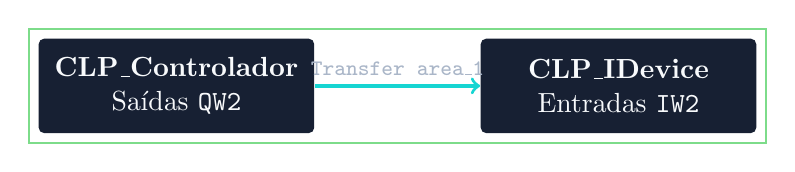
\begin{tikzpicture}
        \node[fill=PanelBg, rounded corners=2pt, minimum width=3.5cm, minimum height=1.2cm, align=center, text=TextPrimary] (ctl) {\textbf{CLP\_Controlador}\\Sa\'idas \texttt{QW2}};
        \node[fill=PanelBg, rounded corners=2pt, minimum width=3.5cm, minimum height=1.2cm, align=center, text=TextPrimary, right=2.1cm of ctl] (dev) {\textbf{CLP\_IDevice}\\Entradas \texttt{IW2}};
        \draw[->, AccentCyan, line width=1.2pt] (ctl) -- node[above, text=TextMuted, font=\footnotesize] {\texttt{Transfer area\_1}} (dev);
        \draw[SignalGreen, line width=0.7pt] ($(ctl.north west)+(-0.12,0.12)$) rectangle ($(dev.south east)+(0.12,-0.12)$);
    \end{tikzpicture}

    \vspace{0.35cm}
    \begin{block}{Resultado esperado}
        O valor escrito em \texttt{QW2} no controlador aparece em \texttt{IW2} no I-Device, via PROFINET RT.
    \end{block}
\end{frame}

\begin{frame}{Fase 3: Assign Device Name}
    \small
    \begin{block}{Por que essa etapa importa?}
        Dispositivos PROFINET n\~ao iniciam a comunica\c{c}\~ao de I/O apenas pelo IP. O controlador precisa associar o \alert{Device Name} ao MAC Address do equipamento f\'isico.
    \end{block}

    \begin{block}{Antes do clique}
        Abrir o Wireshark, selecionar a interface Ethernet do PC e aplicar o filtro:
        \begin{center}
            \Large\texttt{pn\_dcp}
        \end{center}
    \end{block}
\end{frame}

\begin{frame}{DCP no TIA Portal e no Wireshark}
    \small
    \begin{columns}[T,totalwidth=\textwidth]
        \begin{column}{0.46\textwidth}
            \begin{block}{No TIA Portal}
                \begin{itemize}
                    \item Ir para \texttt{Network view}.
                    \item Clicar no \texttt{CLP\_IDevice} ou na rede.
                    \item Selecionar \texttt{Assign device name}.
                    \item Conferir \texttt{PROFINET device name}.
                    \item Selecionar a placa em \texttt{PG/PC interface}.
                    \item Clicar em \texttt{Update list}.
                \end{itemize}
            \end{block}
        \end{column}
        \begin{column}{0.46\textwidth}
            \begin{block}{No Wireshark}
                O \texttt{Update list} dispara pacotes \textit{Identify Request}. O TIA Portal procura equipamentos pelo MAC Address.

                \vspace{0.25cm}
                Depois, selecionar o CLP encontrado e clicar em \texttt{Assign name}.
            \end{block}
        \end{column}
    \end{columns}
\end{frame}

\begin{frame}{Teoria: DCP em Vez de DHCP}
    \small
    \begin{block}{Pergunta para a turma}
        Por que n\~ao usar DHCP, como em celulares e notebooks?
    \end{block}

    \begin{columns}[T,totalwidth=\textwidth]
        \begin{column}{0.46\textwidth}
            \begin{block}{DHCP}
                \begin{itemize}
                    \item Negocia \textit{Discover, Offer, Request, Acknowledge}.
                    \item Pode entregar outro IP.
                    \item Foi pensado para redes de TI.
                \end{itemize}
            \end{block}
        \end{column}
        \begin{column}{0.46\textwidth}
            \begin{block}{DCP}
                \begin{itemize}
                    \item Usa descoberta em camada 2.
                    \item Associa nome de dispositivo ao MAC.
                    \item Reduz tempo de reparo em manuten\c{c}\~ao.
                \end{itemize}
            \end{block}
        \end{column}
    \end{columns}
\end{frame}

\begin{frame}{Camada 2: Unicast, Broadcast e Multicast}
    \small
    \begin{block}{Endere\c{c}o para observar}
        Em pacotes DCP, procure no Wireshark o MAC de destino:
        \begin{center}
            \Large\texttt{01:0E:CF:00:00:00}
        \end{center}
    \end{block}

    \begin{columns}[T,totalwidth=\textwidth]
        \begin{column}{0.30\textwidth}
            \begin{block}{Unicast}
                Um emissor para um receptor.
            \end{block}
        \end{column}
        \begin{column}{0.30\textwidth}
            \begin{block}{Broadcast}
                Um emissor para todos na rede.
            \end{block}
        \end{column}
        \begin{column}{0.30\textwidth}
            \begin{block}{Multicast}
                Um emissor para um grupo espec\'ifico.
            \end{block}
        \end{column}
    \end{columns}
\end{frame}

\begin{frame}{Fase 4: Compila\c{c}\~ao e Download}
    \small
    \begin{block}{Por que baixar hardware e software?}
        A arquitetura mudou: um CLP virou controlador e o outro passou a funcionar como I-Device. O hardware precisa ser carregado novamente.
    \end{block}

    \begin{columns}[T,totalwidth=\textwidth]
        \begin{column}{0.46\textwidth}
            \begin{block}{Controlador}
                \texttt{CLP\_Controlador} $\rightarrow$ \texttt{Download to device} $\rightarrow$ \texttt{Hardware and Software}.
            \end{block}
        \end{column}
        \begin{column}{0.46\textwidth}
            \begin{block}{I-Device}
                Repetir o download no \texttt{CLP\_IDevice}. Parar a CPU se necess\'ario, carregar e colocar em RUN.
            \end{block}
        \end{column}
    \end{columns}

    \vspace{0.25cm}
    \begin{block}{Valida\c{c}\~ao f\'isica}
        LEDs \texttt{ERROR} ou \texttt{MAINT} n\~ao devem piscar. A rede PROFINET deve subir saud\'avel.
    \end{block}
\end{frame}

\begin{frame}{Teoria: Plano de Controle e Plano de Dados}
    \small
    \begin{columns}[T,totalwidth=\textwidth]
        \begin{column}{0.46\textwidth}
            \begin{block}{Plano de controle}
                \begin{itemize}
                    \item Download, configura\c{c}\~ao e diagn\'ostico.
                    \item Usa IP e protocolos mais pesados.
                    \item Ensina \`a rede o que ela deve fazer.
                \end{itemize}
            \end{block}
        \end{column}
        \begin{column}{0.46\textwidth}
            \begin{block}{Plano de dados}
                \begin{itemize}
                    \item Ativo quando as CPUs entram em RUN.
                    \item Fluxo c\'iclico entre \texttt{QW2} e \texttt{IW2}.
                    \item Opera sem a interven\c{c}\~ao do TCP/IP.
                \end{itemize}
            \end{block}
        \end{column}
    \end{columns}

    \vspace{0.35cm}
    \begin{block}{Leitura pr\'atica}
        O download prepara o sistema. O PROFINET RT executa o controle.
    \end{block}
\end{frame}

\begin{frame}{Fase 5: Captura PROFINET RT}
    \small
    \begin{block}{No Wireshark}
        Parar a captura de DCP, trocar o filtro e iniciar uma nova captura:
        \begin{center}
            \Large\texttt{pn\_rt}
        \end{center}
    \end{block}

    \begin{block}{O que deve aparecer}
        Uma sequ\^encia intensa de pacotes, geralmente em ciclos de poucos milissegundos. Em muitos laborat\'orios, o intervalo observado fica pr\'oximo de \alert{2 ms}.
    \end{block}

    \begin{block}{Ponto de prova}
        Ao abrir o pacote, n\~ao h\'a camada IPv4. O frame sai de \texttt{Ethernet II} com EtherType \texttt{0x8892} direto para \texttt{PROFINET IO Real-Time}.
    \end{block}
\end{frame}

\begin{frame}{Determinismo vs. Best Effort}
    \small
    \begin{block}{Pergunta para a turma}
        Por que pular IP e TCP/UDP ajuda o PROFINET RT a ser mais r\'apido?
    \end{block}

    \begin{columns}[T,totalwidth=\textwidth]
        \begin{column}{0.46\textwidth}
            \begin{block}{Ethernet comum}
                \begin{itemize}
                    \item Foco em entregar dados.
                    \item Atraso vari\'avel.
                    \item Melhor esfor\c{c}o.
                \end{itemize}
            \end{block}
        \end{column}
        \begin{column}{0.46\textwidth}
            \begin{block}{Rede industrial}
                \begin{itemize}
                    \item Foco em prazo de entrega.
                    \item Ciclos previs\'iveis.
                    \item Determinismo.
                \end{itemize}
            \end{block}
        \end{column}
    \end{columns}
\end{frame}

\begin{frame}{Anatomia do Frame}
    \small
    \begin{block}{Pacote de TI: ping, web, download}
        \texttt{Ethernet Header} + \texttt{IP Header} + \texttt{TCP/UDP Header} + Dados + \texttt{FCS}
    \end{block}

    \begin{block}{Pacote PROFINET RT}
        \texttt{Ethernet Header} + Dados do CLP + \texttt{FCS}
    \end{block}

    \begin{block}{Conclus\~ao}
        Ao remover IP e TCP/UDP, o CLP evita roteamento, portas l\'ogicas e reordena\c{c}\~ao de pacotes. O dado chega pela interface Ethernet e vai para a mem\'oria de processo.
    \end{block}
\end{frame}

\begin{frame}{QoS e VLAN 802.1Q}
    \small
    \begin{block}{O que abrir no Wireshark}
        Em um pacote \texttt{pn\_rt}, expandir o cabe\c{c}alho \texttt{Ethernet II} e procurar por \texttt{802.1Q Virtual LAN}.
    \end{block}

    \begin{columns}[T,totalwidth=\textwidth]
        \begin{column}{0.46\textwidth}
            \begin{block}{Prioridade}
                O PROFINET RT pode marcar o frame com prioridade \alert{6}. Essa tag informa ao switch que o pacote industrial deve passar antes de tr\'afego comum.
            \end{block}
        \end{column}
        \begin{column}{0.46\textwidth}
            \begin{block}{Efeito}
                Mesmo com tr\'afego TCP pesado na rede, o switch prioriza o ciclo de controle e ajuda a preservar o determinismo.
            \end{block}
        \end{column}
    \end{columns}
\end{frame}

\begin{frame}{Valida\c{c}\~ao L\'ogica}
    \small
    \begin{block}{No controlador}
        Criar uma \textit{Watch Table} no \texttt{CLP\_Controlador} e for\c{c}ar um valor em \texttt{QW2}.
    \end{block}

    \begin{block}{No I-Device}
        Abrir uma \textit{Watch Table} no \texttt{CLP\_IDevice} e observar o mesmo valor chegando em \texttt{IW2}.
    \end{block}

    \begin{block}{Fechamento t\'ecnico}
        O valor observado fecha o ciclo da aula: configura\c{c}\~ao no TIA Portal, tr\'afego capturado no Wireshark e transfer\^encia real de mem\'oria entre CLPs.
    \end{block}
\end{frame}

\begin{frame}{Roteiro de Execu\c{c}\~ao}
    \small
    \begin{columns}[T,totalwidth=\textwidth]
        \begin{column}{0.30\textwidth}
            \begin{block}{15 min}
                Exposi\c{c}\~ao breve: OSI, DCP, RT, QoS e tipos de tr\'afego.
            \end{block}
        \end{column}
        \begin{column}{0.30\textwidth}
            \begin{block}{Pr\'atica}
                Configura\c{c}\~ao no TIA Portal, captura no Wireshark e download nos CLPs.
            \end{block}
        \end{column}
        \begin{column}{0.30\textwidth}
            \begin{block}{10 min}
                Debriefing com o Wireshark: ``est\~ao vendo que n\~ao tem IP aqui?''
            \end{block}
        \end{column}
    \end{columns}

    \vspace{0.35cm}
    \begin{block}{Mensagem final}
        PROFINET RT \'e uma aplica\c{c}\~ao concreta de redes: a decis\~ao de encapsulamento muda lat\^encia, prioridade e previsibilidade.
    \end{block}
\end{frame}

\end{document}
